\begin{frame}{Integrierte Information}
		\begin{columns}
			\alt<1,2>{\begin{column}{0.55\textwidth}
				\begin{itemize}
					\item{Betrachtbar als Speicherung von Information,
						mit Fehlerkorrektur-Mechanismus}
					\item{Integrierte Information für $k$ zufällig ausgewählte
						  14-bit-Folgen}
					\begin{itemize}
						\item{Maximum bei $k \approx 2^{7}$}
					\end{itemize}
				\end{itemize}
			\end{column}
			\begin{column}{0.5\textwidth}
				\centering
				\alt<1>{
\includegraphics[scale=0.14]{graphics/qrcode_whole.jpg}}{}
				\alt<2>{\hspace{-0.08cm}
\includegraphics[scale=0.14]{graphics/qrcode_damaged.jpg}}{}
			\end{column}}{}

		\alt<3>{\begin{column}{0.55\textwidth}
				\begin{itemize}
					\item{Physikalische Systeme}
					\begin{itemize}
						\item{\enquote{Eierkarton}-Potential ($16\times16$)}
						\item{Oben 256 Minima, $S(\text{Grundzustand}) = 8$}
						\item{Unten 16 Minima, $S(\text{Grundzustand}) = 4$}
					\end{itemize}
					\item{Ort $\del{x,y}$ als zwei 4-bit Zahlen: $0_{2} \text{ -- } 15_{2}$}
					\item{Integration}
						\begin{itemize}
							\item{Oben schlecht $\Phi = 0$}
							\item{Unten gut $\Phi = 2$}
						\end{itemize}
				\end{itemize}
			\end{column}
			\begin{column}{0.5\textwidth}
				\centering
				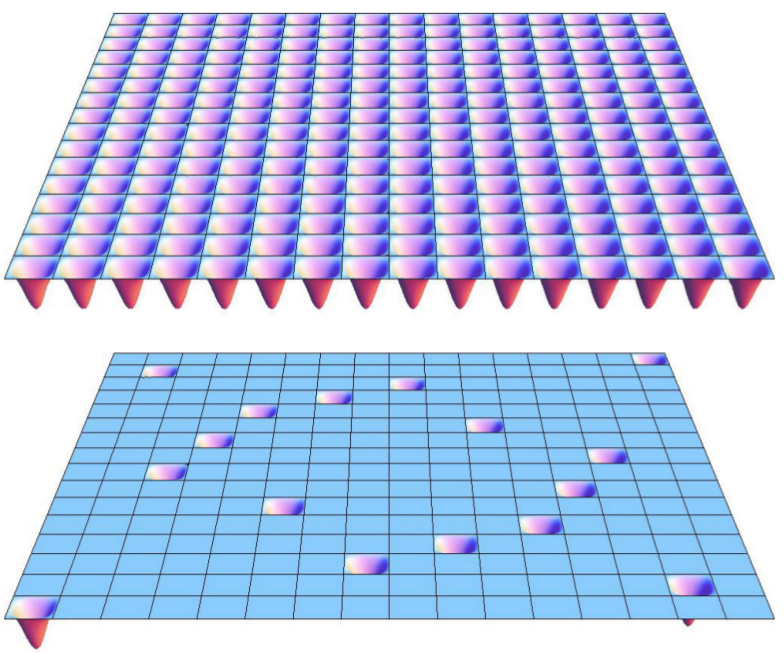
\includegraphics[scale=0.18]{graphics/egg_crate_potentials.jpg}\,\cite{Tegmark_15_long}
			\end{column}}{}	
		\end{columns}
			\centering
			\alt<1,2>{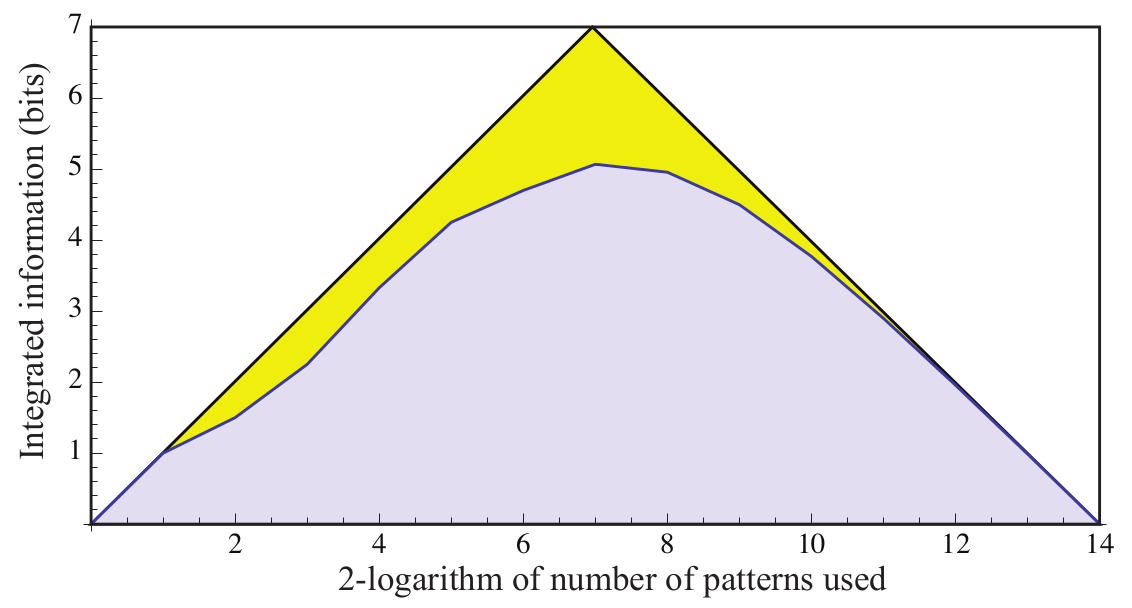
\includegraphics[scale=0.16]{graphics/integrated_information_graph.jpg}\cite{Tegmark_15_long}}{}
\end{frame}